\subsection{Full Stop Tests Results and Discussion}\label{ssec:full-stop-test-results}

		Figure \ref{fig:test-first-ten-snubs} shows a graph with the measured quantities on the first ten of the hundred snubs.

		\begin{figure}[htbp]
				\centering
				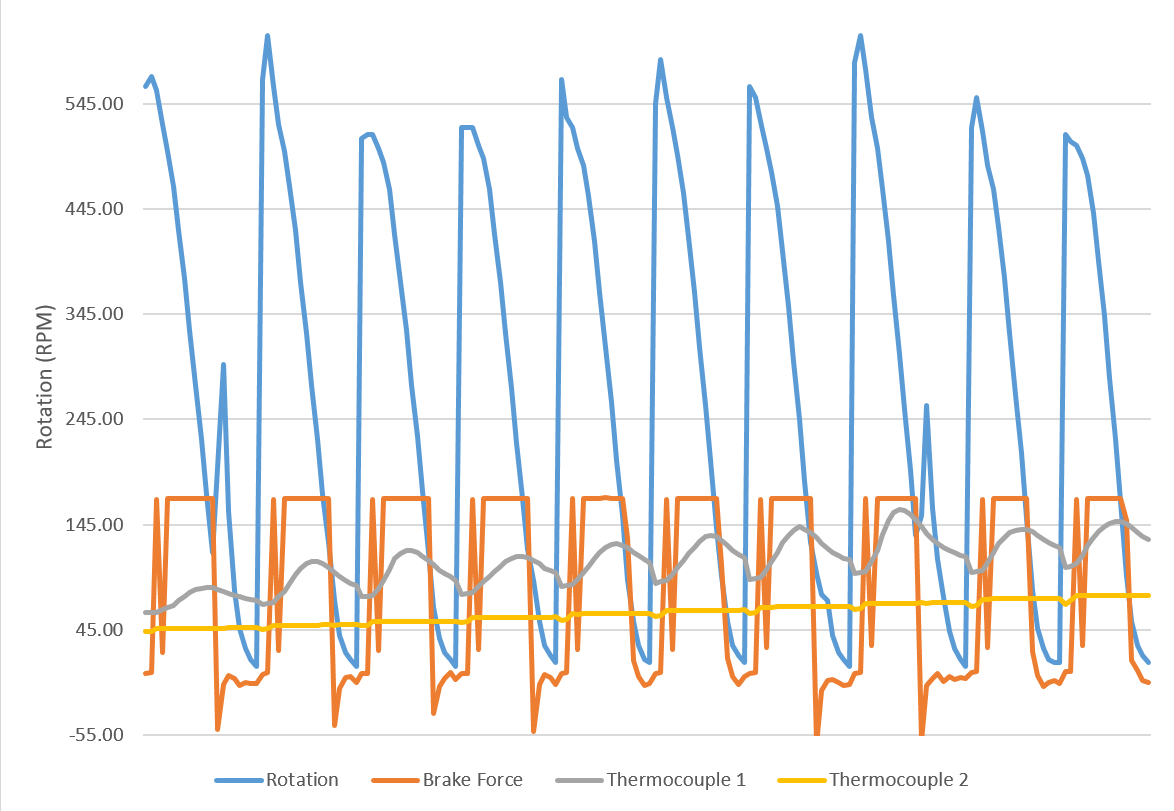
\includegraphics[width=.8\textwidth]{figuras/fig-test-first-ten-snubs}
				\caption{Measurements of the first ten snubs of the test}
				\label{fig:test-first-ten-snubs}
		\end{figure}

		Based on experiment results, it is possible to see the correlation between the measured quantities. Clearly the measured rotation falls rapidly as the brake force saturates to a maximum brake force value. Moreover, at each brake event, detected when the brake force increases, the temperature measured on each of thoose thermocouples increases.
		\par

		Taking a more detailed look at the temperature variation at each snub, Figure \ref{fig:test-first-ten-snubs-force-temperature} show the measured brake force regard the measured temperature at the first ten snubs. This graph states the corelation between the temperature of the brake pads and the braking action, and the fact that the temperature increases during the braking act is perfectly in agreement with the fact that a braking system can be analysed as a kinectic to thermal energy converter, at is was explained in Section \ref{sec:working-principles-of-disk-brake-systems}.

		\begin{figure}[htbp]
				\centering
				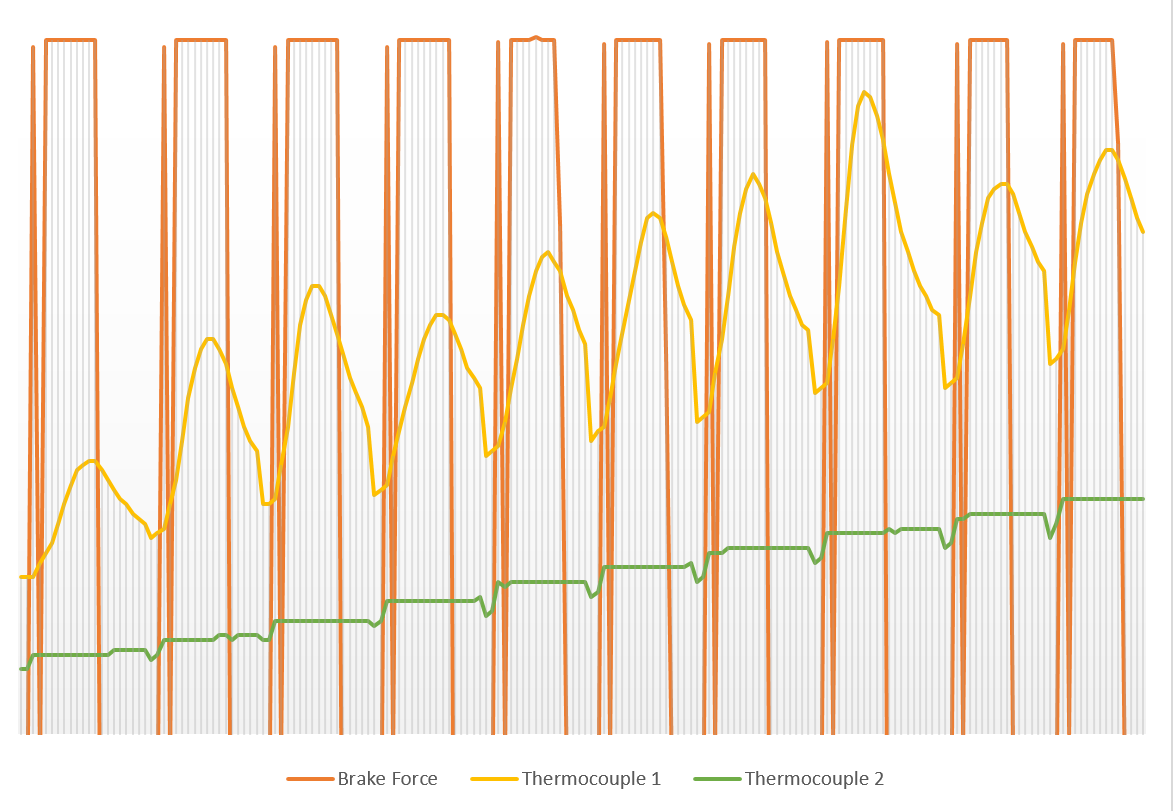
\includegraphics[width=.8\textwidth]{figuras/fig-test-first-ten-snubs-force-temperature}
				\caption{Temperature and Brake Force Measurements of The First Ten Snubs}
				\label{fig:test-first-ten-snubs-force-temperature}
		\end{figure}

		\par

		Whereas the temperature increases at each snub, there may be a point where the temperature reaches a equilibrium, Figure \ref{fig:test-temperature} shows the variation of temperature during the 100 snubs, it is possible to see that even that the temperature bounces at each snub, there may be a point were the temperature stabilizes close to a certain temperature.

		\begin{figure}[htbp]
				\centering
				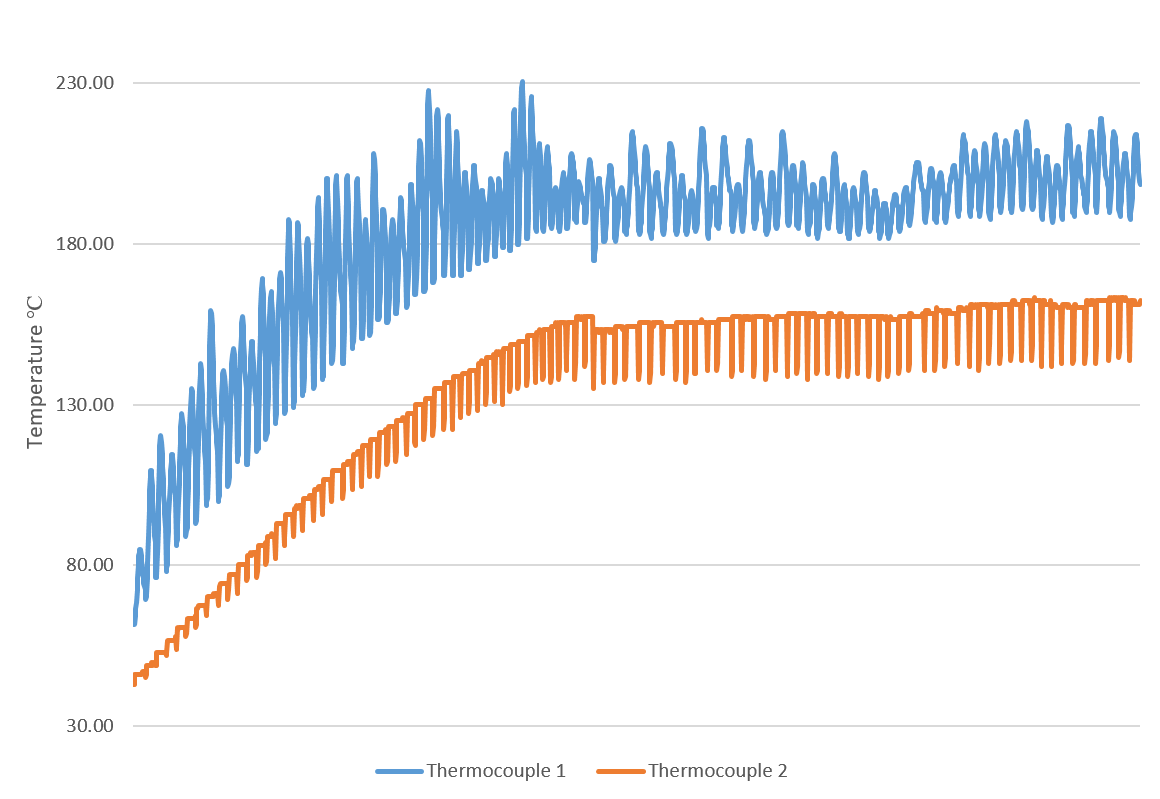
\includegraphics[width=.8\textwidth]{figuras/fig-test-temperature}
				\caption{Temperature Variation During The Whole Test}
				\label{fig:test-temperature}
		\end{figure}
		\par

		Another interesting point to analyse is the effect of the temperature of the pads and the rate of desaceleration of the rotor. Figure \ref{fig:snubs-rotation} shows the desaceleration curves at each snub and shows that during the test the brake efficiency was slightly reduced as the temperature would increase.

		\begin{figure}[htbp]
				\centering
				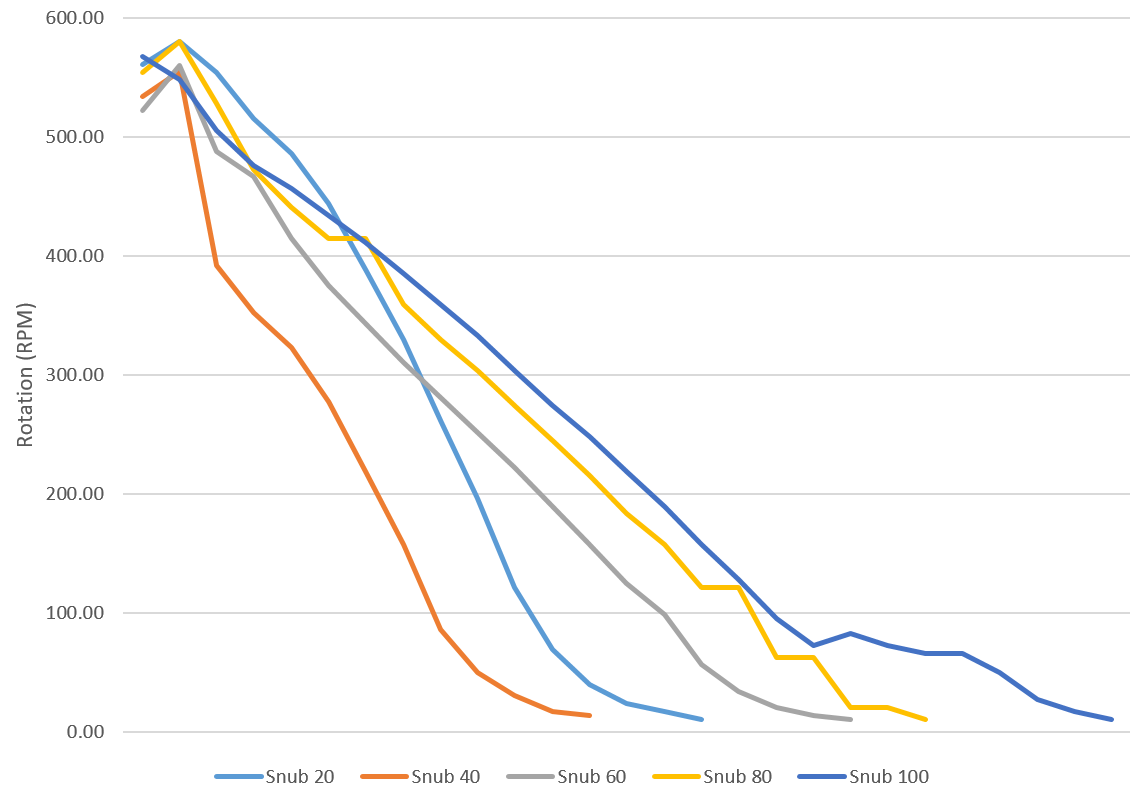
\includegraphics[width=.8\textwidth]{figuras/fig-snubs-rotation}
				\caption{Deceleration During the Whole Test}
				\label{fig:snubs-rotation}
		\end{figure}